\chapter{Decision Support Systems}
\markright{Decision Support Systems}
\renewcommand\textbullet{\ensuremath{\bullet}}
\label{ChapterTwo}
\indent A decision support system (DSS) can be defined as a computer information system that analyzes complex data and solves problems by either supporting decision makers make informed decisions or suggesting decisions/actions for them.\cite{shim2002past} DSSs are a sub-collection of information management systems that help planners, analyzers and managers in the decision making process.\cite{khodashahri2013decision} A decision support system may present information graphically and may include an expert system or artificial intelligence (AI). It may be aimed at business executives or some other group of knowledge workers.
\section{History of Decision support systems}
\label{sec:HistoryOfDecisionSupportSystems}
\indent DSS concept was first introduced in the early 1960s.\cite{power2007brief} A model-oriented DSS or management decision systems was introduced as a new type of information system. The concept of decision support evolved into two main areas of research according to the two DSS pioneers, Peter Keen and Charles Stabell, the first being "the theoretical studies of organizational decision making done at the Carnegie Institute of Technology during the late 1950s and early '60s and the second is the technical work on interactive computer systems, mainly carried out at the Massachusetts Institute of Technology in the 1960s.\cite{power2007brief}\cite{shim2002past}

\indent In 1971, a ground breaking book "Management Decision Systems: Computer-Based Support for Decision Making" written by Michael S. Scott Morton was published. The book discussed how creating analytical models along with computers can help make key decisions. The book also highlighted an experiment where managers used a Management Decision System which was considered the first test of a model-driven decision support system.\cite{power2007brief}

\indent By 1975, J. D. C. Little defined the four main criteria for designing and evaluating models and systems to support management decision making which are still considered relevant today. They include: robustness, ease of control, simplicity, and completeness of relevant detail.\cite{power2007brief} In the early 1990s, some desktop online analytical processing (OLAP) tools were introduced and DSS technology shifted from mainframe-based DSS to client/server-based DSS and eventually to web-based DSS.\cite{bhargava2001decision} As a result of that change, Enterprise data warehouses were completed and data management and decision support companies updated their infrastructure to support the change in DSS technology.

\indent According to Powell \cite{powell2001dm}, DBMS(Database Management systems) vendors "recognized that decision support was different from OLTP(Online transaction processing) and started implementing real OLAP capabilities into their databases". in 1995, Researchers were directed to the development of Web-Based GDSS, Web access to data warehouses in addition to Web-Based and ModelDriven DSS.

According to Power\cite{power2007brief}, in the early 2000's, portals were introduced that combined information portals, knowledge management, business intelligence, and communications-driven DSS in an integrated Web environment called "Enterprise knowledge portals". This solidified the notion that the Web is the best suited platform for building DSS.
\section{Concept of DSS}
\label{sec:FoundationsConcept}
\indent The original DSS concept was built by combining some categories of management activity and decision problem types according to Gorry and Scott Morton.\cite{gorry1989framework} The management activities were the set of decisions defined by the management to serve a specific purpose which could be strategic planning (Decisions that contribute to the overall mission and goals), management control (Decisions guiding the organization to achieve the specified goals), or operational control (decisions directing specific everyday tasks). The decision problem types were categorized into structured, semi-structured or unstructured problems. Structured problem types are problems that are repetitive and easily solved, they are usually solved using a computer program. Unstructured problems are problems that are difficult to solve using a computer program and relies on the decision maker's judgment.\cite{shim2002past}

\indent According to Gorry and Scott Morton the characteristics of information needs and models differ in a DSS environment. The unstructured nature of information needs in DSS situations forces us to search for different kinds of database systems than those for operational environments. Flexible query languages and relational databases are needed. Similarly, the need for flexible modeling environments was arisen to handle the problem of unstructured decision process, such as those in spreadsheet packages.\cite{shim2002past}

\indent Fig. 2.1 explains a generic model that was used and implemented in a DSS system for a decision making process where the focus is on the analysis of the problem and development of the model. It starts by recognizing a problem, then defining said problem in terms that contribute towards the model creation. Once the problem is defined, a model is designed and some alternatives are developed to find a solutions. Once a solution is chosen, the DSS system implements it. This Figure explains a the process of a simple structured clear decision process, however, no decision process is that defined which leads to a lot of back and forth between the phases and overlapping to earlier stages as the problem becomes more defined or the solutions fail.\cite{shim2002past}
\begin{figure}[H]
\centering
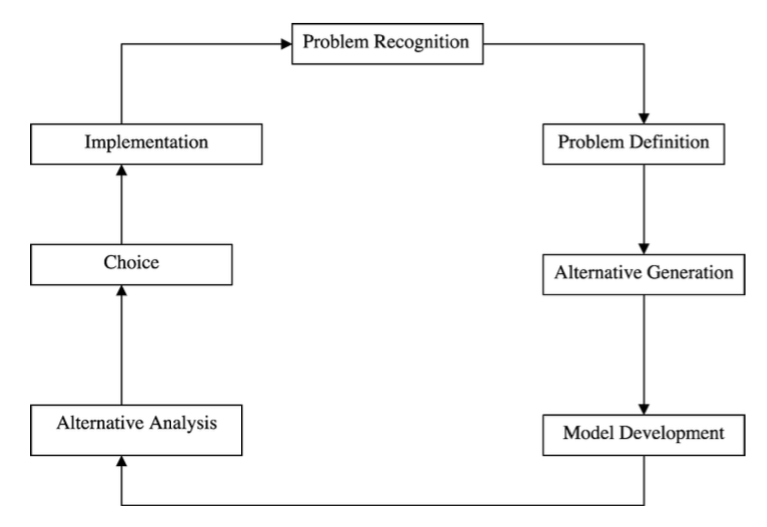
\includegraphics[scale=0.4]{Images/decisionSuppotProcess.png}
\caption[The DSS decision-making process]{The DSS decision-making process \cite{shim2002past}}
\end{figure}
\section{Types of DSS}
\label{sub:TypesOfDSS}
There exists a number of Decision Support Systems. These can be categorized into five types:
\begin{itemize} 
	\item Communication-driven DSS  
	\item Data-driven DSS 
	\item Document-driven DSS 
	\item Knowledge-driven DSS 
	\item Model-driven DSS 
\end{itemize} 
We will explore each type briefly in the following sections.
\subsection{Communication-driven DSS}
\label{subsec:CommunicationDrivenDSS}
\indent A communication-driven DSS is a type of DSS that focuses on communication as well as help two or more users collaborate, share information, co-ordinate their activities and support shared decision-making support.\cite{DDSTypes}The most common technology used to deploy the DSS is a web or client server. A few example of a communication-driven DSS include chats and instant messaging softwares, online collaboration and net-meeting systems or a simple bulletin board or threaded email.

\indent Communications-Driven DSS software should include at least one of the following characteristics:
\begin{itemize}
	\item Enables communication between groups of people
	\item Facilitates information sharing
	\item Supports collaboration and coordination between people
	\item Supports group decision tasks
\end{itemize}
% \paragraph{Group DSS}
% \label{subsubsubsec:GroupDSS}	
\textbf{Group Decision Support Systems(GDSS)} is a hybrid type of DSS. It is based on communication-driven DSS. Using various software tools, multiple users can work collaboratively in groupwork.\cite{DDSTypes}\\
Examples of group support tools are: 
\begin{itemize}
	\item audio conferencing
	\item bulletin boards and web-conferencing
	\item document sharing
	\item electronic mail
	\item computer supported face-to-face meeting software 
	\item interactive video
\end{itemize}
\subsection{Data-driven DSS}
\label{subsec:DataDrivenDSS}
\indent Data-driven DSS is a type of DSS that is able to process huge amounts of data from different sources and store them in a data warehouse system. Data Driven DSS uses on-line analytical processing(OLAP) and Data mining techniques to extract the needed data.\cite{DDSTypes} There exists two special purpose Data-driven DSS, they are: Executive Information Systems (EIS) and Geographic Information Systems (GIS). An example of a data-driven DSS is computer-based databases that have a query system.

\indent Data warehouse systems are systems that allow the manipulation of data by using either computerized tools customized for a specific task or general tools and operators that provide a certain functionality. A Data Warehouse is basically a database that is designed to support decision making in organizations. Data warehouses are structured to contain large amounts of data and handle rapid online queries and managerial summaries. According to Power\cite{power2007brief}, Data warehouse is a subject-oriented, integrated, time-variant, nonvolatile collection of data in support of management's decision making process.

\indent On-line Analytical Processing (OLAP) is a technique used to support the decision support functionality. It is linked to analysis of large collections of historical data.\cite{DDSTypes} OLAP software is used for manipulating data from a variety of sources that has been stored in a static data warehouse. The software can create various views and representations of the data.\cite{DDSTypes} Three main features should be available in a software product for it to be considered an OLAP application. They are: 
\begin{itemize}
\item Multidimensional views of data
\item Complex calculations
\item Time oriented processing capabilities
\end{itemize}
\indent Data Mining helps in extracting useful information by finding patterns or rules from existing data to produce data content relationships. This information is then used to predict future trends and behaviors which also makes it a very important technique when implementing a data-driven DSS.

\indent Executive Information Systems (EIS) are computerized systems intended to provide current and appropriate information to support executive decision making for managers using a networked workstation. They focus on graphical displays and on offering an easy to use interface that presents information from the corporate database. EIS offer strong reporting and drill-down capabilities.\cite{DDSTypes}

\indent A Geographic Information System (GIS) or Spatial DSS is a support system that represents data using maps. It helps people access, display and analyze data that have geographic content and meaning.\cite{DDSTypes}
\subsection{Document-driven DSS}
\label{subsec:DocumentDrivenDSS}
A relatively new field in Decision Support is Document-Driven DSS. Its focus is on the retrieval and management of unstructured documents. Documents can be Oral, written or video. They help a decision maker by keeping track of knowledge that is represented as documents that can affect the decisions.\cite{power2002building} Examples of oral documents are conversations that are transcribed; video can be news clips, or television commercials; written documents can be written reports, catalogs, letters from customers, memos, and even e-mail.\cite{DDSTypes}
\subsection{Knowledge-driven DSS}
\label{subsec:KnowledgeDrivenDSS}
Knowledge-Driven DSS can suggest or recommend actions to managers. It contains of specialized problem solving expertise also known as a knowledge base. The knowledge base comprises of rules, facts and procedures about a particular domain. The knowledge base also provides understanding of problems within that domain, and "skill" for solving some of these problems. A related technique used in knowledge-driven DSS is Data Mining, previously discussed. Intelligent Decision Support methods are used to build Knowledge-Driven DSS  \cite{power2002building}.
\subsection{Model-driven DSS}
\label{subsec:ModelDrivenDSS}
Model-Driven DSS (MDS) are a standalone systems that performs modeling of unstructured problems with an easy to use user interface. The most basic modeling functionality; the what-if model ;can be achieved using a simple statistical and analytical tool. There can exist a hybrid DSS system that combines the modeling functionality of the MDS and the complex analysis of data of an OLAP system.\cite{DDSTypes} In general, model-driven DSS use complex financial, simulation, optimization or multi-criteria models to provide decision support.\cite{DDSTypes} Data and parameters are provided by decision makers to the Model-driven DSS to aid decision makers in analyzing a situation. Very large data bases are not needed in Model-driven DSS as they are not usually data intensive.\cite{DDSTypes} Early versions of Model-Driven DSS were called Computationally Oriented DSS by Bonczek, Holsapple and Whinston (1981) \cite{bonczek1981generalized,power2002building} as well as model-oriented or model-based decision support systems.\\
Tools used in Model-driven DSS include \cite{makowski2003modeling}:
\begin{itemize}
	\item \textbf{Decision Analysis tools} - help decision makers decompose and structure problems. These tools aim to help a user apply models like decision trees, multi-attribute utility models, Bayesian models, Analytical Hierarchy Process (AHP), and related models.\cite{DDSTypes}
	\item \textbf{Forecasting Support System} - A computer-based system that supports users in making and evaluating forecasts. Users can analyze a time series of data.\cite{DDSTypes}
	\item \textbf{Linear Programming} - A mathematical model for optimal solution of resource allocation problems.\cite{DDSTypes}
	\item \textbf{Simulation} - A technique for conducting one or more experiments that test various outcomes resulting from a quantitative model of a system.\cite{DDSTypes}
\end{itemize}
% \section{Functionality}
% \label{sec:Functionality}
\section{Interfaces}
\label{sec:Interfaces}
\indent Classic DSS tool design is comprised of components for (i) sophisticated database management capabilities with access to internal and external data, information, and knowledge, (ii) powerful modeling functions accessed by a model management system, and (iii) powerful, yet simple user interface designs that enable interactive queries, reporting, and graphing functions. Much research and practical design effort has been conducted in each of these domains.\\

\section{Implementation}
\label{sec:Implementation}

\section{Evaluation and Impact}
\label{sec:EvaluationAndImpact}